\chapter{Kuinka järjestelmä hajautetaan?}
\begin{it}
	Kirjoita tähän yleistä tietoa tästä kappaleesta. Tietona ulos tulee lukijalle mitä tässä kappaleessa käsitellään kokonaisuudessaan. Tämän voisi kijoittaa viimeisenä.
\end{it}
Aikaisemmin käsiteltiin erilaisia hajautuksen paradigmoja ja kuinka osapuolet voivat kommunikoida hajautetussa järjestelmässä. Tässä kappaleessa analysoidaan näitä paradigmoja ja arvoidaan mitkä sopisivat tässä työssä suunniteltavan ohjelmistokomponentin tarkoituksiin. Lisäksi käsitellään avointa AMQP-kommunikointistandardia (engl. Advanced Message Queing Protocol), joka mahdollistaa erilaisten hajautusparadigmojen toteutuksen osapuolten välillä. AMQP:stä käsitellään sen toiminnallisuutta ja kuinka se sopii tämän työn tarpeisiin.

% TODO: Kirjoita tämä vastaamaan muuta tekstiä kun muut kappaleet ovat valmiit.


\section{Arkkitehtuurin analyysi}
\label{ch:architecture-analysis}
IEC 61850 -standardi määrittää, että viestit IED-laitteelta tulevat julkaisija-tilaaja-pa\-ra\-dig\-man mukaisesti. Viestit tilataan IED-laitteelta olevilta RCB-luokkien instansseilta. RCB-instanssi on kytketty laitteella olevaan datajoukkoon, jonka tiedoista ollaan kiinnostuneita. Rajoituksena standardi asetti, että RCB-instanssi täytyy tilaajan varata ja yksi RCB-instanssi voi palvella vai yhtä tilaajaa kerrallaan. RCB-instansseja IED-laitteissa on rajallinen määrä yhtä datajoukkoa kohti ja näitä voidaan myös käyttää aseman sisäiseen toimintaan. Tässä työssä käsitellyssä IED-laitteessa yhteen datajoukkoon oli esimerkiksi määritetty viisi eri RCB-instanssia. Seurauksena on, että kyseisen datajoukon voi tilata vain viisi saman aikaista tilaajaa. Lisäksi tässä työssä testattu IED-laite rajoitti avoimet yhteydet viiteen. Tästä ylimeneviä yhteyksiä ei avattu ja IED-laite palautti standardin mukaisen negatiivisen vastauksen.

Vaatimuksissa määriteltiin että IED-laitteen tieto täytyy saada jaettua järjetelmän muiden komponenttien kanssa. Työn tekohetkellä komponentteja järjestelmässä oli kaksi. Mittaustiedon näyttämiseen ja tilatiedon tarkkailuun. Vaatimuksissa kuitenkin määriteltiin, että toteutuksessa haluttiin varautua tulevaisuuden varalle komponenttien suhteen. Eli tilanteeseen jossa niitä olisi enemmän kuin kaksi ja niiden määrä voisi vaihtua tilaamisen aloitusten välillä. 

Edelle mainituista IED-laitteen rajoituksista ja työlle asetetuista vaatimuksista voidaan tehdä johtopäätöksiä hajautuksen arkkitehtuurin suhteen. Samalle IED-laitteelle avattujen yhteyksien määrä halutaan pitää pienenä. Tämän lisäksi varattujen RCB-instanssien määrä jokaista datajoukkoa kohti halutaan myös pitää pienenä. Nämä sen takia, koska halutaan mahdollisimman vähän varata aseman resursseja sen muulta käytöltä. Lisäksi järjestelmän IED-laitteelta vaatimat resurssit halutaan pitää ennalta määrättynä lukuna. Tämä helpottaa aseman insinöörin suunnittelutyötä, koska hän voi ottaa luvut huomioon IED-laitteiden konfiguroinnissa.

Edellä mainittuun tilanteeseen ratkaisuna voisi ajatella, että järjestelmän yksittäiset komponentit tilaisivat niiden tarvitsemat tiedot suoraan IED-laitteelta. Tämä on esitetty kuvan \ref{fig:architecture-analysis} yläosassa. Ongelmana tässä kuitenkin on aikaisemmin mainittu yhteyksien määrän rajoitus IED-laitteelle ja niiden määrä haluttiin minimoida ja pitää vakiona. Lisäksi viestit tilataan ja palautetaan komponentille MMS-protokollamäärityksien mukaisesti. Seurauksena on, että jokainen komponentti joutuu käsittelemään MMS-protokollan binääridataa itse tai kirjaston avulla. Viestin muoto olisi parempi olla ymmärrettävämpi. Näin viestin lukeminen eri tekniikoilla olisi helpompaa. Tämä asetettiin ohjelmiston vaatimuksissa ja oli myös yksi kohta työlle asetetuista tutkimuskysymksistä.

\begin{figure}[ht!]
	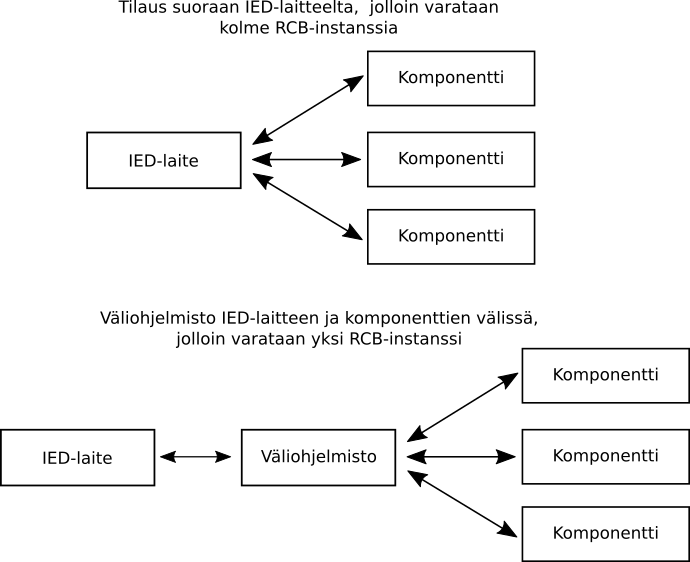
\includegraphics[width=0.7\textwidth]{pictures/architecture-analysis.png}
	\caption{IED-laitteelta viestien tilaus suoraan ja väliohjelmiston avulla.}
	\label{fig:architecture-analysis}
\end{figure}

Ratkaisuna edellä mainittuun tilanteeseen on kommunikoinnin epäsuoruuden lisääminen. Samoin menee myös kuuluisa lainaus henkilöltä David Wheeler \cite[s.~290]{beautiful-code}:
\begin{quote}
	All problems in computer science can be solved by another level of indirection.
\end{quote}
Epäsuoruutta saadaan aikaan toteuttamalla erillinen ohjelmistokomponentti IED-laitteen ja muiden järjestelmän komponenttien väliin. Tätä komponenttia voisi kutsua myös nimellä \emph{väliohjelmisto} (engl. \emph{middleware}) ja on esitetty kuvan \ref{fig:architecture-analysis} alaosassa. Väliohjelmisto tilaisi viestit IED-laitteelta ja halutuilta RCB-instansseilta. Samalla komponentti muokkaisi saapuvat viestit parempaan muotoon, joka olisi helpompi muiden järjestelmän komponenttien lukea. Väliohjelmiston avulla yhteyksien määrä IED-laitetta kohti saadaan yhteen. Tämän avulla myös saadaan minimoitua varattujen RCB-instanssien määrä datajoukkoa kohti yhteen. Tuloksena on vakiomäärät yhteyksiä ja RCB-istansseja datajoukkoa kohti jotka ovat helpompi ennustaa ja konfiguroida etukäteen tarpeiden mukaan.

Vaatimuksissa mainittiin myös, että muu järjestelmä ohjaa viestien tilauksen aloittamista ja lopettamista. Väliohjelmistoa on mahdollista muun järjestelmän ohjata tarvittavin tilauksien mukaan. Tietysti tieto tilauksesta täytyy myös saada järjestelmän muille komponenteille. Väliohjelmisto ja epäsuoruus myös helpottavat viestien puskuroinnin toteuttamista komponenteille, joka myös oli vaatimuksena. Ilman epäsuoruutta, jokaisen komponentin pitäisi toteuttaa oma sisäinen puskuri viestien vastaanottamiseen.

Tässä kappaleessa analysoitiin IEC 61850 -standardin asettamia rajoja ja ohjelmistolle asetettuja vaatimuksia. Näistä analysoitiin mikä olisi toimiva ratkaisu tässä tilanteessa järjestelmän hajauttamiseen korkealla tasolla. Tuloksena järjestelmään päätettiin lisätä epäsuoruutta toteuttamalla väliohjelmisto IED-laitteen ja järjestelmän muiden komponenttien väliin. Tämän jälkeen täytyy vielä miettiä mitkä kommunikointiparadigmat toteuttavat väliohjelmiston ja komponenttien vaatimukset? Mihin muotoon MMS-tason viesti väliohjelmistossa pitäisi muuttaa jakoa varten? Mitkä ovat väliohjelmiston ja muiden komponenttien väliset liitoksien vahvuudet? Kuinka viestien puskurointi väliohjelmiston avulla toteutetaan?


\section{Osapuolten liitoksien analyysi}
Aikaisemmin kappaleessa \ref{ch:liitokset} käsiteltiin hajautetun järjestelmän osapuolten välisiä liitoksia. Erilaiset liitoksien luokittelut esiteltiin taulukossa \ref{tab:communication-models}. Lisäksi hajautetussa järjestelmässä kommunikointi osapuolten välillä voi olla suoraan tai epäsuoraa. Aikaisemmin kappaleessa \ref{ch:architecture-analysis} päädyttiin lisämään epäsuoruutta IED-laitteen ja järjestelmän muiden komponenttien väliin.

IED-laitteen ja viestien tilaajan välinen kommunikointi on suoraa ja se ei tapahtu välikäden kautta. Lisäksi osapuolten välillä on vahva tila- ja aikaliitos. Tilaliitos tulee kun kummatkin osapuolet tietävät toistensa identiteetin (IP-osoitteen). Aikaliitoksessa osapuolien täytyy olla olemassa samaan aikaan. Tilaajan täytyy olla ottamassa viesti vastaan kun IED-laite viestin lähettää ja IED-laitteen täytyy olla olemassa kun tilaus tehdään. Kaikki edellemainitut tulevat IEC 61850 -standardin määrityksien seurauksena ja näihin ei työn puitteissa voi vaikuttaa.

Työn aloitushetkellä järjestelmässä oli kaksi tietoa tarvitsevaa komponenttia. Vaatimusten mukaan haluttiin varautua tulevaisuuten, jossa niitä voisi olla enemmänkin. Tästä seurauksena väliohjelmiston ja muiden järjestelmän komponenttien välinen suhde on yksi-moneen. Vaatimuksena oli, että tietoa tarvitsevien komponenttien määrä pystyisi muuttumaan tilauksien välillä. Toteuttamalla suora kommunikointi väliohjelmiston ja järjestelmän muiden komponenttien väliin. Väliohjelmiston tarvitsee tietää muiden komponenttien olemassaolosta ja kenelle viestit täytyy ohjata. Tämä lisäisi osapuolten välistä riippuvuutta ja vähentäisi toteutuksen joustavuutta. Ratkaisuna on lisätä epäsuoruutta väliohjelmiston ja muiden komponenttien väliin välikädellä. Tämä on esitetty kuvassa \ref{fig:coupling-analysis}. Välikäsi vähentää osapuolten välistä riippuvuutta ja lisää toteutuksen joustavuutta. Se myös auttaa toteuttamaan asetettuja vaatimuksia, kuten viestien puskurointia ja uuden viestin ilmoitusta. Vaatimuksena oli, että IED-laitteelta tulevaa tietoa pitäisi pystyä jakamaan komponenteille IED-laitteen perusteella. Välikäden tuoma epäsuoruus auttaa myös tämän vaatimuksen toteuttamisessa. Tällä vastuu väliohjelmistolta viestien jakamisesta saadaan siirrettyä välikäden vastuulle.

\begin{figure}[ht!]
	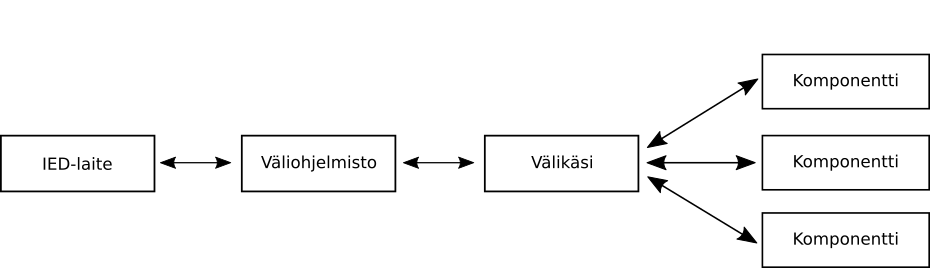
\includegraphics[width=1\textwidth]{pictures/coupling-analysis.png}
	\caption{Välikäsi väliohjelmiston ja komponenttien välissä lisämään epäsuoruutta ja joustavuutta.}
	\label{fig:coupling-analysis}
\end{figure}

Väliohjelmiston ja muiden komponenttien välille edellä mainitun perusteella halutaan heikko tilaliitos. Väliohjelmiston ei tarvitse tietää järjestelmän muiden komponenttien identiteettiä ja tämä parantaa toteutuksen joustavuutta. Aikaliitos asetettujen vaatimuksien perusteella pystyisi olemaan vahva tai heikko. Kuitenkin muu järjestelmä ohjaa tilauksen aloittamista, jolloin muutkin komponentit tietävät asiasta. Tämä vaatimus poistaa tarpeen heikolle aikaliitokselle.

Tässä kappaleessa analysoitiin hajautetussa järjestelmässä osapuolten välisi liitoksien vahvuutta. IEC 61850 -standardi asettaa rajoitteet IED-laitteen ja väliohjelmiston välille, joihin ei voida vaikuttaa. Väliohjelmiston ja muiden komponenttien väliin päädyttiin toteuttamaan epäsuora kommunikointi joustavuuden ja vaatimusten takia. Samojen osapuolten väliin halutiin toteuttaa heikko tilaliitos ja vahva aikaliitos. Kysymyksenä jää miettiä millä hajautuksen paradigmoilla välikäsi pitäisi toteuttaa, jotta halutut ominaisuudet saadaan toteutettua?


\section{Paradigmojen analyysi}
Aikaisemmissa kappaleissa analyysien ja vaatimusten pohjalta päädyttiin kuvan \ref{fig:coupling-analysis} hajautetun järjestelmän arkkitehtuuriin. Tässä kappaleessa vertaillaan ja analysoidaan eri hajautuksen paradigmoja. Tarkoituksena on selvittää mitä paradigmoja tarvitaan, jotta asetetut vaatimukset voidaan toteuttaa. Näitä olivat viestien puskurointi, ilmoitukset komponenteille uuden viestin saapuessa ja viestien suodattamisen mahdollisuus IED-laitteen mukaan. Tässä kappaleessa käsitellyt paradigmat koskevat kuvan \ref{fig:coupling-analysis} välikättä väliohjelmiston ja järjestelmän komponenttien välissä. Hajautetun järjestelmän eri paradigmat oli esitetty taulukossa \ref{tab:communication-paradigms}.

Järjestelmään haluttiin epäsuoruutta välikädellä. Tätä parhaiten tarjoavat epäsuorat kommunikointiparadigmat. Vaatimuksena oli, että viestejä pitäisi pystyä puskuroimaan myöhempään ajan hetkeen jos komponentti ei niitä ehdi käsitellä. Tämän ominaisuuden parhaiten tarjoaa viestijonoparadigma. Viestejä haluttiin erotella IED-laitteen mukaan, ja komponentit voisivat päättää itse mistä ovat kiinnostuneita. Tätä ominaisuutta epäsuorista paragidmoista tarjoavat joukkokommunikointi ja julkaisija-tilaaja. Joukkokommunikoinnissa komponentti pystyisi olemaan osa haluttuja ryhmiä. Julkaisija-tilaaja-paradigmassa komponentti pystyisi tilaamaan halutut viestit. Kummatkin edellä mainituista tarjoavat myös haluttut ilmoitukset. Joukkokommunikointi- ja julkaisija-tilaaja-systeemissä vastaanottajat saavat ilmoituksen uuden viesti saapuessa. Jotta joukkokommunikoinilla saadaan haluttu toiminnallisuus, pitää ryhmän olla avoin ja sen pitää mahdollistaa osapuolten liittyminen ja poistuminen ryhmästä. Lisäksi ryhmien pitää sallia olevan päällekkäisiä. Tämän sen takia, että komponenttin on mahdollisesti saada viestejä useammasta lähteestä samaan aikaan.

Järjestelmään halutun epäsuoruuden takia suorat kommunikointiparadigmat eivät sovellu kovin hyvin hajautuksen toteuttamiseen. Näitä olivat prosessien välinen kommunikointi ja etäkutsut. Hajautuksessa osapuolien välillä haluttiin olevan heikko tilaliitos ja vahva aikaliitos. Kummassakin edellä mainitussa paradigmassa liitokset ovat vahvoja. Suoralla kommunikoinnilla vastaanottavan osapuolen pitäisi toteuttaa viestipuskuri itse, verrattuna jos käytettävä epäsuora systeemi tarjoaisi puskurin sen sijaan. Tämä hankaloittaa uusien komponenttien kehitystyötä. Muu järjestelmä on toteutettu web-applikaationa, josta seurasi vaatimus, että kommunikoinnin pitäisi toimia TCP/IP-protokollaperheen päällä tai vastaavalla. Prosessien välinen kommunikointi tapahtuu mm. soketeilla ja näin ollen on vaatimukseen nähden liian matalaa. Etäkutsut tarjovat tähän paremman vaihtoehdon, mutta vaatimuksissa ei ollut tarvetta pyyntö-vastaus-kommunikoinnille. Viestien suunta on tässä tapauksessa yhden suuntaista IED-laitteelta järjestelmän komponentille.

Asetettuihin vaatimuksiin nähden epäsuorat paradigmat sopivat toteutukseen parhaiten. Näistä tarvitaan viestijono-paradigmaa viestien puskurointiin ja joukkokommunikointi tai julkaisija-tilaaja niiden lähettämiseen komponenteille. Joukkokommunikointi ja julkaisija-tilaaja paradigmat ovat kummatkin tilanteeseen sopivia vaihtoehtoja. Jäljelle jää miettiä millä tekniikalla halutut paradigmat toteutetaan. Valitun tekniikan pitäisi yhdistää kaksi eri paradigmaa niin, että viestien oikea reitittäminen ja puskurointi ovat mahdollisia.

% TODO: Miettiä onko muita syitä hylätä joukkokommunikointi vaihtoehtona kuin tekniikan valinta.


\section{Toteutuksien analyysi}
Hajautetun järjestelmän toteuttamiseen löytyy erilaisia avoimia standardeja kuten \emph{AMQP} (engl. \emph{Advanced Message Queuing Protocol}) \cite{amqp-homepage} ja \emph{MQTT} (engl. \emph{Message Queuing Telemetry Transport}) \cite{mqtt-homepage}. Standardien tarkoitus on määrittää yhteiset säännöt osapuolten kommunikointiin hajautetussa järjestelmässä. Standardien pohjalta on toteutettu erilaisia viestien välitysohjelmistoja, johon muut osapuolet voivat ottaa yhteyttä standardin mukaisesti tekniikasta riippumatta. Kummatkin edellä mainitut standardit ovat määritetty toimivaksi TCP/IP-protokollaperheen päällä \cite[s.~1]{mqtt-specification} \cite[s.~22]{AMQP-specification}.

MQTT on julkaisija-tilaaja-paradigmaan pohjautuva kommunikointistandardi. MQTT\--mää\-ri\-tyk\-si\-en mukainen välittäjäpalvelin tarjoaa myös viestien puskuroinnin mahdollisuuden \cite{mqtt-specification}. MQTT on pääasiassa tarkoitettu kommunikointiin, missä kaista on rajallista ja kommunikoinnista huolehtivan koodin jalanjälki täytyy olla pientä. Tästä syytä se on paljon käytetty standardi IoT-laitteissa (engl. Internet of Things) ja kotiautomaatiossa \cite[s.~9--11]{mqtt-for-iot}.

AMQP-standari on tarkoitettu MOM:in toteuttamiseen (engl. Message-Oriented Middleware) ja näin ollen mahdollistaa monen eri kommunikointiparadigman toteuttamisen \cite[s.~6]{AMQP-specification}. MOM tarkoittaa hajautetussa järjestelmässä \emph{väliohjelmistoa} (middleware), jota käytetään lähettämään ja vastaanottamaan viestejä. MOM:in tarkoitus on tarjota heterogeeninen alusta viestien vaihtoon tekniikasta ja verkkoprotokollasta riippumatta \cite{mom}. AMQP-standardi mahdollistaa esimerkiksi viestijonot, etäkutsut ja erilaiset reititykset kuten pisteestä pisteeseen ja julkaisija-tilaaja. AMQP tarjoaa toteutukseen enemmän paradigma vaihtoehtoja kuin MQTT.

Tässä työssä toteutuksen tekniikaksi valittiin AMQP. AMQP tarjoaa kaikki vaaditut ominaisuudet välikäden toteuttamiseen. AMQP ei mahdollista joukkokommunikoinnin toteuttamista, mutta mahdollistaa julkaisija-tilaaja-paradigman. Aikaisemmin julkaisija-ti\-laa\-ja-paradigma todettiin toteutukseen sopivaksi vaihtoehdoksi joukkokommunikoinnin kanssa. AMQP tarjoaa viestien puskuroinnin jokaista tilaaja kohden ja komponenttien on mahdollista myös suodattaa viestejä kiinnostuksensa mukaan. MQTT olisi myös todennäköisesti sopinut toteutukseen, koska se tarjosi kaikki vaaditut ominaisuudet. Työssä kuitenkin päädyttiin AMQP:n valintaan tekijän aikaisemman kokemuksen ja muiden työntekijöiden keskustelun tuloksena. Viestien lähetykselle järjestelmässä ei vaadittu takuita, mutta nämä olisi hyvä olla olemassa tulevaisuuden takia. AMQP tarjoaa takuumekanismit viestien lähettämiseen transaktioina ja vastaanottamiseen niiden kuittaamisella \cite[s.~14,21]{AMQP-specification}.


\section{Viestin formaatti}
IED-laitteelle kommunikointi ja siltä tulevat viestit esitetään MMS-protokollan binäärimäärityksien mukaan. Jotta viestin sisältö olisi helppo tilaavien komponenttien lukea, täytyy se muuntaa toiseen muotoon. Hajautetussa järjestelmässä viestejä voidaan lähettää lähettäjän formaatin tai yhteisen hyväksytyn formaatin mukaan. Jos viestin lähettäjä päättää formaatin, täytyy viestissä olla tieto sen muodosta, jotta vastaanottaja on mahdollista se lukea. Järjestelmän yhteisessä formaatissa tätä tietoa ei tarvia, koska kaikki osapuolet käytävät samaa formaattia ilman poikkeuksia. Viestejä voidaan lähettää binääri- tai tekstimuodossa. Binäärimuodossa datarakenteet esitetään binääreinä ja tekstimuodossa ne esitetään tekstimuodossa. Tekstimuoto on yleensä pitempi esitysmuoto kuin binäärimuoto.

Aikaisempien kappaleiden pohjalta päädyttiin kuvan \ref{fig:coupling-analysis} pohjaiseen arkkitehtuuriin. Arkkitehtuurissa väliohjelmiston tehtävä on tilata viestejä IED-laitteelta, muutta ne ymmärrettävään muotoon ja julkaista AMQP-välittäjäpalvelimelle. Järjestelmän komponentit tilaavat viestejä AMQP-palvelimelta tarpeidensa mukaan.

Järjestelmän komponenteille viestin lukeminen haluttiin pitää helppona ja viestin koolla ei ollut teknisiä rajoitteita. Tämän takia viestit päätetiin esittää mielummin tekstiformaatissa. Tekstimuoto on helpompi ihmisen lukea esimerkiksi vikatilanteissa. Binääritiedon lukeminen yleensä tarvitsee erillisen ohjelman. Nykypäivänä web-teknologioissa on käytössä kaksi tunnettua tekstimuotoista esitystapaa, joita ovat \emph{XML} (engl. \emph{Extensible Markup Language)}) \cite{xml-specification} ja \emph{JSON} (engl. \emph{JavaScript Object Notation}) \cite{json-standard}.

Työssä viestien välityksen tekniikaksi valittiin JSON. JSON on nopeampi ja kevyempi tiedonsiirtoformaatti kuin XML \cite{json-xml-comparison}. Lisäksi JSON on nykypäivänä paljon käytetty tiedonsiirron muoto web-rajapinnoissa kuten REST (engl. Representational State Transfer). JSON:in lukemin ihmiselle on helppoa ja sille on olemassa tuki valmiina monelle eri ohjelmointikielelle ilman erillistä kirjastoa. JSON on myös kasvattunut suosiotaan ajan saatossa XML:lään verrattuna \cite{google-trends-xml-json}. Ja asiasta on kirjoitettu erilaisia blogiposteja kuten \cite{the-rise-and-rise-of-json, why-json-is-better-than-xml, Patrizio2016}.